\chapter{Continuous Hopfield Neural Networks}
\label{ch:CHopfield}

Because a Hopfield neural network works on discrete input, its process is discontinuous. This can make it difficult to use in a continuous problem, such as classifying photos of cats and dogs, or in a feed-forward neural network.

\noindent In this chapter we introduce continuous Hopfield neural networks, following on from the article \cite{ramsauer2021hopfieldnetworksneed}. These neural networks accept real values and update them with continuous and derivable transformations. This way it's possible to use them in continuous problems and train the neural networks to get good patterns for a data set.

\section{Derivation}
%% recall era scritto racall
In \cref{ch:DHopfield} we define a discrete Hopfield neural network as a predictor that receives an input in $\{-1,+1\}^d$ and recovers a pattern in the same space.

\noindent We denoted the patterns to be recovered as $x_1,\ldots,x_P \in \{-1,+1\}^N$ or using the matrix $X\in\mathbb{R}^{N\times P}$ in general, the current state as $\xi$ and a sequence of states as $(\xi^t)_t$.

\noindent We have defined the energy $E\left(\xi,X\right) = -\sum_{i}^{P} F\left(\xi^Tx_i\right)$ and the asynchronous update:
\begin{align*}
	\xi^{\text{new}}_j &\mathdef \sgn \left[\sum_{i=1}^{P}F\left(x_{ij}+\sum_{l\neq j}x_{il}\xi_l\right)-F\left(-x_{ij}+\sum_{l\neq j}x_{il}\xi_l\right)\right] \\
	&= \sgn \left[-E\left(\xi\,|\,\xi_j=1,X\right)+E\left(\xi\,|\,\xi_j=-1,X\right)\right]
\end{align*}

\noindent The mean value theorem gives a value $v\in\left[-1,1\right]$ such that:
\begin{equation}
    E\left(\xi\,|\,\xi_j=1,X\right)-E\left(\xi\,|\,\xi_j=-1,X\right) = 2\frac{\partial E\left(\xi,X\right)}{\partial \xi_j}\left(\xi\,|\,\xi_j=v,X\right)
\end{equation}

\noindent To derive the continuous Hopfield neural network we use the interaction function $F:x\mapsto e^{\beta x}$, where $\beta^{-1}$ is called \textbf{temperature}, a positive value. Thus the updating formulation can be written from \cref{def:discupdating} as
\begin{align}
\xi^{\text{new}}_j &= \sgn \left[-E\left(\xi\,|\,\xi_j=1,X\right)+E\left(\xi\,|\,\xi_j=-1,X\right)\right] \nonumber \\
&= \sgn \left[\exp\left(\ln\left(\sum_{i=1}^{P} \exp\left(\beta\left(\xi\,|\,\xi_j=1\right)^Tx_i\right)\right)\right)-\exp\left(\ln\left(\sum_{i=1}^{P} \exp\left(\beta\left(\xi\,|\,\xi_j=-1\right)^Tx_i\right)\right)\right)\right] \nonumber \\
&= \sgn \left[\beta^{-1}\ln\left(\sum_{i=1}^{P} \exp\left(\beta\left(\xi\,|\,\xi_j=1\right)^Tx_i\right)\right)-\beta^{-1}\ln\left(\sum_{i=1}^{P} \exp\left(\beta\left(\xi\,|\,\xi_j=-1\right)^Tx_i\right)\right)\right] \label{eq:energy_derivation} \\
&= \sgn \left[2\frac{\partial E\left(\xi,X\right)}{\partial \xi_j}\left(\xi\,|\,\xi_j=v,X\right)\right]
= \sgn \left[\frac{\sum_{i=1}^{P}x_{ij}\exp\left(\beta\left(\xi\,|\,\xi_j=v\right)^Tx_i\right)}{\sum_{k=1}^{P}\exp\left(\beta\left(\xi\,|\,\xi_j=v\right)^Tx_k\right)}\right] \nonumber \\
&= \sgn \left[\left[X\softmax\left(X^T\left(\beta\xi\,|\,\xi_j=v\right)\right)\right]_j\right] \label{eq:update_derivation}
\end{align}
Hence, in general $\xi^{\text{new}} = \sgn \left[X\softmax\left(X^T\left(\beta\xi\,|\,\xi_j=v\right)\right)\right]$

\bigskip In view of the above, let us define a Continuous Hopfield Neural Network according to the following definitions:
\begin{definition}[Energy]
    We define the energy using \cref{eq:energy_derivation} as
    \begin{equation*}
        E_\beta\left(\xi,X\right) = -\beta^{-1}\ln\left(\sum_{i=1}^{P} \exp\left(\beta\xi^Tx_i\right)\right) + \frac12\xi^T\xi + \const = -\lse\left(\beta, X^T\xi\right) + \frac12\xi^T\xi + \const
    \end{equation*}
    we observe that: $\left(\xi\,|\,\xi_j=1\right)^T\left(\xi\,|\,\xi_j=1\right) = \left(\xi\,|\,\xi_j=-1\right)^T\left(\xi\,|\,\xi_j=-1\right)$.

    \noindent To achieve more specific properties, we say:
    \begin{equation}
        E_\beta\left(\xi,X\right) = -\lse\left(\beta, X^T\xi\right) + \frac12\xi^T\xi + \beta^{-1}\ln P + \frac12 M^2
    \end{equation}
    where $M^2 = \max \|x_i\|^2$
\end{definition}
\begin{definition}[updating]
    \label{def:updating}
    We define the update using \cref{eq:update_derivation} as
    \begin{equation}
        \label{eq:updating}
        \xi^{\text{new}} = X\softmax\left(\beta X^T\xi\right)
    \end{equation}
\end{definition}

\section{Properties}
%% property era scritto al plurale
A first simple property is:
\begin{equation}
\label{eq:energy_simply}
E_\beta\left(\xi,X\right) = -\beta^{-1}\ln\left[\frac{1}{P}\sum_{i=1}^{P}\exp\left(-\frac12\beta\|\xi-x_i\|^2\right)\exp\left(-\frac12\beta\left(M^2-\|x_i\|^2\right)\right)\right]
\end{equation}
This formula emphasises that the energy uses the density of $P$ symmetric Gaussian variables chosen with equal probability but with different centres.

\noindent Using \cref{eq:energy_simply} it's easy to prove the following lemma:
\begin{lemma}[energy lower bound]\text{from Lemma.A1 in \cite{ramsauer2021hopfieldnetworksneed}}\\
    For all states, the energy is formally non-negative:
    \[
        \forall\xi\in\mathbb{R}^N\left(E_\beta\left(\xi,X\right)\geq0\right)
    \]
    \begin{proof}
        For all $\xi\in\mathbb{R}^N$, it holds that:
        \begin{align*}
            E_\beta\left(\xi,X\right)\geq0 &\iff \frac{1}{P}\sum_{i=1}^{P}\exp\left(-\frac12\beta\|\xi-x_i\|^2\right)\exp\left(-\frac12\beta\left(M^2-\|x_i\|^2\right)\right) \leq 1 \\
            &\impliedby \forall{i\in\{1,\ldots,P\}} \left(\exp\left(-\frac12\beta\|\xi-x_i\|^2\right)\exp\left(-\frac12\beta\left(M^2-\|x_i\|^2\right)\right)\leq1\right) \\
            &\iff \forall{i\in\{1,\ldots,P\}} \left(\left(-\frac12\beta\|\xi-x_i\|^2\right)+\left(-\frac12\beta\left(M^2-\|x_i\|^2\right)\right)\leq0\right) \\
            &\iff \forall{i\in\{1,\ldots,P\}} \left(\|\xi-x_i\|^2+\left(M^2-\|x_i\|^2\right)\geq0\right) \\
        \end{align*}
    \end{proof}
\end{lemma}
A second simple property is that the vector \textbf{softmax} in \cref{eq:updating} is a probability distribution. Let $p \mathdef \left(p_1,\ldots,p_P\right)=\softmax\left(\beta X^T\xi\right)$, the new state $\xi^{\text{new}}$ is a convex combination of the patterns in $X$:
\[
\xi^{\text{new}} = Xp = p_1x_1+\cdots+p_Px_P
\]
With $\langle{x_1,\ldots,x_P}\rangle$ the set $\{v|\exists p_1,\ldots,p_P\left(v=p_1x_1+\cdots+p_Px_P\right)\}$.

\noindent Hence the sequence $\xi^1,\xi^2,\ldots\in\langle{x_1,\ldots,x_P}\rangle$. Now we compute an upper bound for the energy, whether or not it is temperature dependent.
\begin{lemma}[energy upper bound] \text{from Lemma.A1 in \cite{ramsauer2021hopfieldnetworksneed}}\\
    For all $\xi\in\langle{x_1,\ldots,x_P}\rangle$, it holds that:
    \begin{itemize}[itemsep=2pt, topsep=10pt]
        \item[i)]
        $E_\beta\left(\xi,X\right)\leq2 M^2$
        \item[ii)] $E_\beta\left(\xi,X\right)\leq\beta^{-1}\ln P + \frac12 M^2$
    \end{itemize}
    \begin{proof}
        $\exp$ is a convex function over $\mathbb{R}$ so, for all $v_1,\ldots,v_P\in\mathbb{R}$, it holds that:
        \begin{itemize}[itemsep=2pt, topsep=10pt]
            \item $\forall{p_1,\ldots,p_P}\geq0\left(p_1+\cdots+p_P=1\implies\sum_{i=1}^{P}p_i\exp\left(v_i\right)\geq\exp\sum_{i=1}^{P}p_iv_i\right)$
            \item $\forall{p_1,\ldots,p_P}\geq0\left(p_1+\ldots+p_P=1\implies\max_i\exp\left(v_i\right)\geq\exp\sum_{i=1}^{P}p_iv_i\right)$
        \end{itemize}

        \noindent Proof of the first relation:
        \begin{align*}
            E_\beta\left(\xi,X\right) &= -\beta^{-1}\ln\left(\sum_{i=1}^{P}\exp\left(\beta X^T\xi\right)\right) + \frac12\xi^T\xi + \beta^{-1}\ln P + \frac12 M^2 \\
            &= -\beta^{-1}\ln\left(\frac{1}{P}\sum_{i=1}^{P}\exp\left(\beta\xi^Tx_i\right)\right)+\frac12\xi^T\xi+\frac12M^2 \\
            &\leq -\beta^{-1}\left(\frac{1}{P}\sum_{i=1}^{P}\beta\xi^Tx_i\right)+\frac12\xi^T\xi+\frac12M^2 \\
            &= -\xi^Tm_x + \frac12\xi^T\xi+\frac12M^2 \leq \|\xi\|\,\|m_x\| + \frac12\|\xi\|^2+\frac12M^2\leq2M^2
        \end{align*}
        using $m_x \mathdef \frac{1}{P}\sum_{i=1}^{P}x_i $

        \noindent Proof of the second relation:

        \noindent Let $p_1,\ldots,p_P\geq0$ be such that $p_1+\cdots+p_P=1$ and $\xi=\sum_{i=1}^{P}p_ix_i$.
        \begin{align*}
            E_\beta\left(\xi,X\right) &= -\beta^{-1}\ln\left(\sum_{i=1}^{P}\exp\left(\beta\xi^Tx_i\right)\right) + \frac12\xi^T\xi + \beta^{-1}\ln P + \frac12 M^2 \\
            &\leq -\beta^{-1}\ln\left(\max_i\exp\left(\beta\xi^Tx_i\right)\right) + \frac12\xi^T\xi + \beta^{-1}\ln P + \frac12 M^2 \\
            &\leq -\beta^{-1}\sum_{i=1}^{P}p_i\beta\xi^Tx_i + \frac12\xi^T\xi + \beta^{-1}\ln P + \frac12 M^2 \\
            &= - \frac12\xi^T\xi + \beta^{-1}\ln P + \frac12 M^2 \leq \beta^{-1}\ln P + \frac12 M^2
        \end{align*}
    \end{proof}
\end{lemma}

\subsection{Convergence}
Before we talk about convergence, we observe some simple properties of the energy minimization problem. Now we will talk about the $\lse$ function:
\begin{remark}
\text{from Lemma.22 in \cite{ramsauer2021hopfieldnetworksneed}}\\
    The Jacobian of $\softmax$ is positive semi-definite matrix.
    \begin{align*}
        \nabla_{v_i}\left[\softmax\left(v\right)\right]_j &= \nabla_{v_i}\frac{\exp v_j}{\sum_{k=1}^{P}\exp v_k} = \frac{\left(\nabla_{v_i}\exp v_j\right)\sum_{k=1}^{P}\exp v_k-\exp v_j\nabla_{v_i}\sum_{k=1}^{P}\exp v_k}{\left(\sum_{k=1}^{P}\exp v_k\right)^2} \\
        &= \frac{\delta_{ij}\exp v_i\sum_{k=1}^{P}\exp v_k-\exp v_j\exp v_i}{\left(\sum_{k=1}^{P}\exp v_k\right)^2} = \delta_{ij}\frac{\exp v_i}{\sum_{k=1}^{P}\exp v_k}-\frac{\exp v_j\exp v_i}{\left(\sum_{k=1}^{P}\exp v_k\right)^2}
    \end{align*}
    Hence, if we define $p(v)=\softmax\left(v\right)$:
    \[
        \nabla_{v}p(v) = \diagonal(p(v))-p(v)p(v)^T
    \]
    Proof that the Jacobian of $\softmax$ has eigenvalue zero with eigenvector $\mathds{1}$:
    \[
        \nabla_{v}p(v)\mathds{1} = (\diagonal(p(v))-p(v)p(v)^T)\mathds{1} = p(v) - p(v) = 0
    \]
    Furthermore $\forall h \in \mathbb{R}^P $ holds:
     \begin{align*}
         h^T \nabla_{v}p(v) h &= h^T ( \diagonal(p(v))-p(v)p(v)^T ) h = \left(\sum_{k=1}^{P} p(v)_k h_k^2\right)- \left( \sum_{k=1}^P p(v)_k h_k \right)\\
         &= \left(\sum_{k=1}^{P} p(v)_k h_k^2\right)\left(\sum_{k=1}^P p(v)_k \right)- \left( \sum_{k=1}^P p(v)_k h_k \right) \geq 0
     \end{align*}
     where the last inequality is Cauchy-Schwartz applied to $a ,b$ such that $a_k=\sqrt{p(v)_k}h_k$ and $b_k = \sqrt{p(v)_k}$
\end{remark}
\begin{remark}
    The gradient of $\lse\left(\beta, v\right)$ with respect to $v$ is $\softmax(\beta v)$.
    \[
    \nabla_{v_i}\lse\left(\beta, v\right) = \nabla_{v_i}\beta^{-1}\ln\sum_{k=1}^{P}\exp\left(\beta v_k\right) = \frac{\exp\left(\beta v_i\right)}{\sum_{k=1}^{P}\exp\left(\beta v_k\right)} = \left[\softmax(\beta v)\right]_i
    \]
    So the Hessian of $\lse\left(\beta, v\right)$ respect $v$ is positive semi-definite, and so $\lse\left(\beta, v\right)$ is a convex function respecting $v$.
\end{remark}

\noindent The objective function is a sum of convex and concave functions respecting $\xi$:
\begin{equation}
	\label{eq:convex_concave}
	E_\beta\left(\xi,X\right) = E_\beta^{-}\left(\xi,X\right) + E_\beta^{+}\left(\xi,X\right)
\end{equation}
where:
\begin{itemize}[itemsep=2pt, topsep=10pt]
	\item $E_\beta^{-}\left(\xi,X\right) = -\lse\left(\beta, X^T\xi\right)$ a concave function
	\item $E_\beta^{+}\left(\xi,X\right) = \frac12\xi^T\xi + \beta^{-1}\ln P + \frac12 M^2$ a convex function
\end{itemize}
We observe that the objective function does not describe a convex problem, but the domain is the convex $G\mathdef\langle{x_1,\ldots,x_P}\rangle$. We want to prove that the sequence defined in \cref{eq:updating} reduces the energy and converges to local minimum.
\begin{proposition} \text{from Theorem.A1 in \cite{ramsauer2021hopfieldnetworksneed}}\\
	\label{prop:convex_problem}
	The updating formula $\xi^{t+1} = X\softmax\left(X^T\xi^{t}\right)$ solves the problem:
	\[
	\xi^{t+1}\in\argmin_{\xi\in G} \xi^T\nabla_{\xi^{t}}E_\beta^{-}\left(\xi^{t},X\right) + E_\beta^{+}\left(\xi,X\right)
	\]
	\begin{proof}
		This is a convex problem and we can solve it by finding the value where the gradient is zero:
		\[
		\nabla_{\xi}\left(\xi^T\nabla_{\xi^{t}}E_\beta^{-}\left(\xi^{t},X\right) + E_\beta^{+}\left(\xi,X\right)\right) = \nabla_{\xi^{t}}E_\beta^{-}\left(\xi^{t},X\right) + \nabla_{\xi}E_\beta^{+}\left(\xi,X\right) = \nabla_{\xi^{t}}E_\beta^{-}\left(\xi^{t},X\right) + \xi
		\]
		We know that $\nabla_{\xi^{t}}E_\beta^{-}\left(\xi^{t},X\right) = -X\softmax(\beta X^T\xi^t)$, so:
		\[
		0 = \nabla_{\xi}\left(\xi^T\nabla_{\xi^{t}}E_\beta^{-}\left(\xi^{t},X\right) + E_\beta^{+}\left(\xi,X\right)\right) \iff \xi = X\softmax(\beta X^T\xi^t)
		\]
	\end{proof}
\end{proposition}
\begin{remark}
	We can linearize the energy formulation \cref{eq:convex_concave} only over the concave function:
	\[
	f_{\beta}\left(\xi,\xi^{t},X\right) \mathdef E_\beta^{+}\left(\xi,X\right) + E_\beta^{-}\left(\xi^{t},X\right) + \left(\xi-\xi^{t}\right)^T\nabla_{\xi^{t}}E_\beta^{-}\left(\xi^{t},X\right)
	\]
	This function is convex and has other important properties.
\end{remark}
\begin{proposition}[The updating reduces the energy] \text{from Theorem.A1 in \cite{ramsauer2021hopfieldnetworksneed}}\\
	\[
	\forall{t\in\mathbb{N}_0}\left(E_{\beta}\left(\xi^{t+1},X\right)\leq E_{\beta}\left(\xi^{t},X\right)\right)
	\]
	\begin{proof} We noticed that:
		\begin{itemize}[itemsep=2pt, topsep=10pt]
			\item $f_{\beta}\left(v,v,X\right) = E_{\beta}\left(v,X\right)$
			\item $\xi^{t+1}\in\argmin_{\xi\in G} f_{\beta}\left(\xi,\xi^{t},X\right)$ from \cref{prop:convex_problem}
			\item $f_{\beta}\left(v,w,X\right) \geq E_{\beta}\left(v,X\right)$, because $E_{\beta}^{-}\left(v,X\right)$ is concave over $v$ and so:\\
			$E_{\beta}^{-}\left(w,X\right) + \left(v-w\right)^T\nabla_{w}E_\beta^{-}\left(w,X\right) \geq E_\beta^{-}\left(v,X\right)$
		\end{itemize}
		So for all $t\in\mathbb{N}_0$, it holds that:
		\[
		E_{\beta}\left(\xi^{t+1},X\right) \leq f_{\beta}\left(\xi^{t+1},\xi^{t},X\right) \leq f_{\beta}\left(\xi^{t},\xi^{t},X\right) = E_{\beta}\left(\xi^{t},X\right)
		\]
	\end{proof}
\end{proposition}
If the updating reduces the energy and the energy is non-negative, the sequence $\left(E_{\beta}\left(\xi^{t},X\right)\right)_t$ converges to $E^\star$, which depends on the starting point.\\
Furthermore, the sequence of states $\left(\xi^{t}\right)_t$ is a compact set in $G$. So there are accumulation points (denoted as $\xi^\star$) for the sequence of states $\left(\xi^{t}\right)_t$ and for them the energy is $E^\star$.
\begin{theorem}[stationary points] \text{from Theorem.A2 in \cite{ramsauer2021hopfieldnetworksneed}}\\
    \label{th:statonary_points}
    For all states $\xi$, then it holds that:
    \begin{itemize}[itemsep=2pt, topsep=10pt]
        \item $\nabla_{\xi}E_{\beta}\left(\xi,X\right) = 0 \iff \xi = \xi^{\text{new}}$
        \item $E_{\beta}\left(\xi,X\right) = E_{\beta}\left(\xi^{\text{new}},X\right)\iff\xi = \xi^{\text{new}}$
    \end{itemize}
    \begin{proof}
        We observe that the convex problem $\argmin_v f_{\beta}\left(v,w,X\right)$ is the computation of the minimum of a quadratic form, in fact the Hessian of $f$ over $v$ is the identity:
        \[
        \frac{\partial^2 f_{\beta}\left(v,w,X\right)}{\left(\partial v\right)^2} = I_d
        \]
        so the solution is unique in $\mathbb{R}^d$.

        \noindent Let $\xi$ be such that $\nabla_{\xi}E_{\beta}\left(\xi,X\right) = 0$:
        \[
            \nabla_v f_{\beta}\left(v,\xi,X\right)\big|_{v=\xi}=\nabla_v E_{\beta}^{+}\left(v,X\right)\big|_{v=\xi}+\nabla_{\xi} E_{\beta}^{-}\left(\xi,X\right) = \nabla_\xi E_{\beta}\left(\xi,X\right) = 0
        \]
        so $\xi$ is a valid solution and so is the unique solution, hence $\xi^{\text{new}} = \xi$.

        \noindent Let $\xi$ be such that $\xi^{\text{new}} = \xi$:
        \[
            0 = \nabla_v f_{\beta}\left(v,\xi,X\right)\big|_{v=\xi}=\nabla_v E_{\beta}^{+}\left(v,X\right)\big|_{v=\xi}+\nabla_{\xi} E_{\beta}^{-}\left(\xi,X\right) = \nabla_\xi E_{\beta}\left(\xi,X\right)
        \]
        so $\xi$ is a stationary points, hence $\nabla_\xi E_{\beta}\left(\xi,X\right) = 0$.\\ Furthermore, is obviously that $E_{\beta}\left(\xi,X\right) = E_{\beta}\left(\xi^{\text{new}},X\right)$ if $\xi = \xi^{\text{new}}$

        \noindent Let $\xi$ be such that $\xi^{\text{new}} \neq \xi$. Since the result of the convex problem is unique, then:
        \[
            E_{\beta}\left(\xi^{\text{next}},X\right) \leq f_{\beta}\left(\xi^{\text{next}},\xi,X\right) < f_{\beta}\left(\xi,\xi,X\right) = E_{\beta}\left(\xi,X\right)
        \]
        Hence, the statement of this theorem holds.
    \end{proof}
\end{theorem}
\begin{lemma}
    \label{lemma:sequences}
    Let a sequence $\left(v_n\right)_n$ be such that $2 \leq |\accumulation\{v_n\}_n| < \infty$.
    \[
        \exists v_1^\star, v_2^\star \in \accumulation\{v_n\}_n \ \exists \left(v_{n_i}\right)_i\subseteq\left(v_n\right)_n\left(v_{n_i} \to v_1^\star \land v_{n_i+1} \to v_2^\star \land v_1^\star\neq v_2^\star\right)
    \]
    \begin{proof}

        \noindent Get a sequence $\left(v_{n_i^j}\right)_i$ for each accumulation point $v^j \in \accumulation\{v_n\}_n$.

        \noindent Without loss of generality $\forall i,a\exists j,b\left(a\neq b \land n_i^a+1=n_j^b\right)$

        \noindent Let $S \mathdef \{v^j\}_j\times\{v^j\}_j$ be the set of couples of accumulation points.

        \noindent Let $h:(a,b)\in{S}\to|\{i\in\mathbb{N}|n_i^a+1=n_i^b\}|\in\mathbb{N}_\infty$ be a counter of jumps from sub-sequence of $v^a$ to sub-sequence of $v^b$. Clearly $\forall a\left(h(a,a)=0\right)$ and $\sum_{a,b\in{S}}h\left(a,b\right)=\infty$.

        \noindent Let $a,b$ be such that $a\neq b$ and $h\left(a,b\right)=\infty$, so there exists a sub-sequence $\left(n_{i_k}^a\right)_k\subseteq\left(n_i^a\right)$ such that $\left(n_{i_k}^a+1\right)_k\subseteq\left(n_i^b\right)_i$.

        \noindent In this way $v_{n_{i_k}^a} \to v^a$ and $v_{n_{i_k}^a+1} \to v^b$
    \end{proof}
\end{lemma}
\begin{theorem}[accumulation points] \text{from Theorem.A2 in \cite{ramsauer2021hopfieldnetworksneed}}\\
	\label{th:acc_pt}
	\[
	|\accumulation\{\xi^t\}_t| < \infty \implies \accumulation\{\xi^t\}_t=\{\xi^\star\} \land \nabla_{\xi^\star}E_{\beta}\left(\xi^\star,X\right) = 0
	\]
	\begin{proof}
		\textbf{Ad absurdum} $|\accumulation\{\xi^t\}_t| \geq 2$.\\
		\noindent Let $\xi^\star_1, \xi^\star_2$ be different accumulation points such that $\exists \left(\xi^{t_i}\right)_i\subseteq\left(\xi^t\right)_t\left(\xi^{t_i} \to \xi_1^\star \land \xi^{t_i+1} \to \xi_2^\star\right)$ (see \cref{lemma:sequences}).

		\noindent Get $2$ sub-sequences of $\left(\xi^t\right)_t$ over indexing $(n_i)_i$, $(m_i)_i$ such that:
		\begin{itemize}[itemsep=2pt, topsep=10pt]
			\item $m_i = n_i+1$
			\item $\xi_{n_i} \to \xi^\star_1$, $i \to \infty$
			\item $\xi_{m_i} \to \xi^\star_2$, $i \to \infty$
		\end{itemize}
		For all $i\in\mathbb{N}_0$ hold $\xi_{m_i} = \xi_{n_i+1} = X\softmax\left(\beta X^T\xi_{n_i}\right)$, hence $\xi^\star_2 = X\softmax\left(\beta X^T\xi^\star_1\right)$

		\noindent We already know that $E^\star=E_{\beta}\left(\xi^\star_1,X\right) = E_{\beta}\left(\xi^\star_2,X\right)$

		\noindent With \cref{th:statonary_points} it holds that $\xi^\star_1 = \xi^\star_2 \;\;\text{\Lightning}$

		\bigskip\noindent It is proved that ${\accumulation\{\xi^t\}_t} = \{\xi^\star\}$

		\noindent The sub-sequence $\left(\xi^{t+1}\right)_t$ converges to $\xi^\star$.

		\noindent Hence $\xi^\star = X\softmax\left(\beta X^T\xi^\star\right)$ and finally $\nabla_{\xi}E_{\beta}\left(\xi^\star,X\right) = 0$ (using \cref{th:statonary_points}).
	\end{proof}
\end{theorem}
\begin{corollary}
	The \cref{th:acc_pt} also proves that the local energy minima are separated and that the sequence starting at $\xi^0$ converges to one of them.
\end{corollary}

\section{Analysis}
We have proved that given a starting point $\xi_0$ the sequence defined by the updating rule converges to some minimum of the energy; the next question to analyze is whether the starting point has an influence on the point of convergence.\\
To study this, we write the updating rule as:
$\xi^{\text{new}} = f(\xi)$. From a previous remark we can compute the Jacobian of $f$ as:
\[
J = \frac{\partial f(\xi)}{\partial \xi} = \beta X \left(\diagonal(p(\beta X^T \xi)) - p(\beta X^T \xi)p(\beta X^T \xi)^T \right)X^T = \beta J_s
\]
From now on we write $p = p(\beta X^T \xi)$ to simplify the notation. \\
We also write: $\mathbb{E}_p\left[f(x)\right] = \sum_i p_i f(x_i)$.
\begin{lemma}
    $\textnormal{Var}_p(x) = J_s$
    \begin{proof}
        \begin{align*}
            \text{Var}_p\left(x\right) &= \mathbb{E}_p\left[xx^T\right] - \mathbb{E}_p\left[x\right] \mathbb{E}_p\left[x\right]^T = X \mathbb{E}_p\left[\mathds{1}\right]X^T - Xp (Xp)^T \\
            &= X(\diagonal(p))X^T -  Xp (Xp)^T =
            X(\diagonal(p) - p p^T) X^T = J_s
        \end{align*}
        where the last equality holds for a remark made in the previous section.
    \end{proof}
\end{lemma}
The parameter $\beta$ plays a central role in the convergence of the method; in fact, if its value is too high, the softmax result is similar to a uniform distribution for any given input, and this can cause the network to lose information about the input.
\begin{definition}
    We define:
    \begin{align*}
        &m_X = \frac1N \sum x^i \quad \textbf{patterns mean} \\
        &\bar{m} = \sum p_i x^i \quad \textbf{patterns weighted mean} \\
        &m^2_{\max} = \max_i \left\|x^i - m_X\right\|^2
    \end{align*}
\end{definition}
\begin{proposition}\text{from lemma.A3 in \cite{ramsauer2021hopfieldnetworksneed}}\\
\label{prop:J_norm}
    $$\left\|J\right\|_2< \beta m^2_{\max} $$

    \noindent So if $\beta m^2_{\max} < 1 $, the sequence defined by the continuous Hopfield neural network converges to a fixed point for any given input.
    \begin{proof}
        \begin{align*}
            \left\|J_s\right\|_2 &= \left\|\text{Var}_p\left(x\right)\right\|_2 = \left\|\mathbb{E}_p\left[(x - \bar{m})(x - \bar{m})^T\right]\right\|_2 = \left\|\sum_i p_i (x^i - \bar{m})(x^i - \bar{m})^T\right\|_2\\
            &\leq \sum_i p_i \left\|(x^i - \bar{m})(x^i - \bar{m})^T\right\|_2 = \sum_i p_i \left\|x^i - \bar{m}\right\|^2 \leq \sum_i p_i \left\|x^i - m_X\right\|^2 \leq m^2_{\max}
        \end{align*}
        where in the penultimate inequality we used:
        \begin{align*}
            \min_m \sum_i p_i \left\|x^i - m\right\|^2 = \sum_i p_i \left\|x^i - \bar{m}\right\|^2
        \end{align*}
        To prove the second part of the statement we can use the Banach fixed point theorem and note that the sequence defined by the network is inside the compact set  $\langle{x_1,\ldots,x_P}\rangle$
    \end{proof}
\end{proposition}

\begin{figure}[hb]
    \centering
    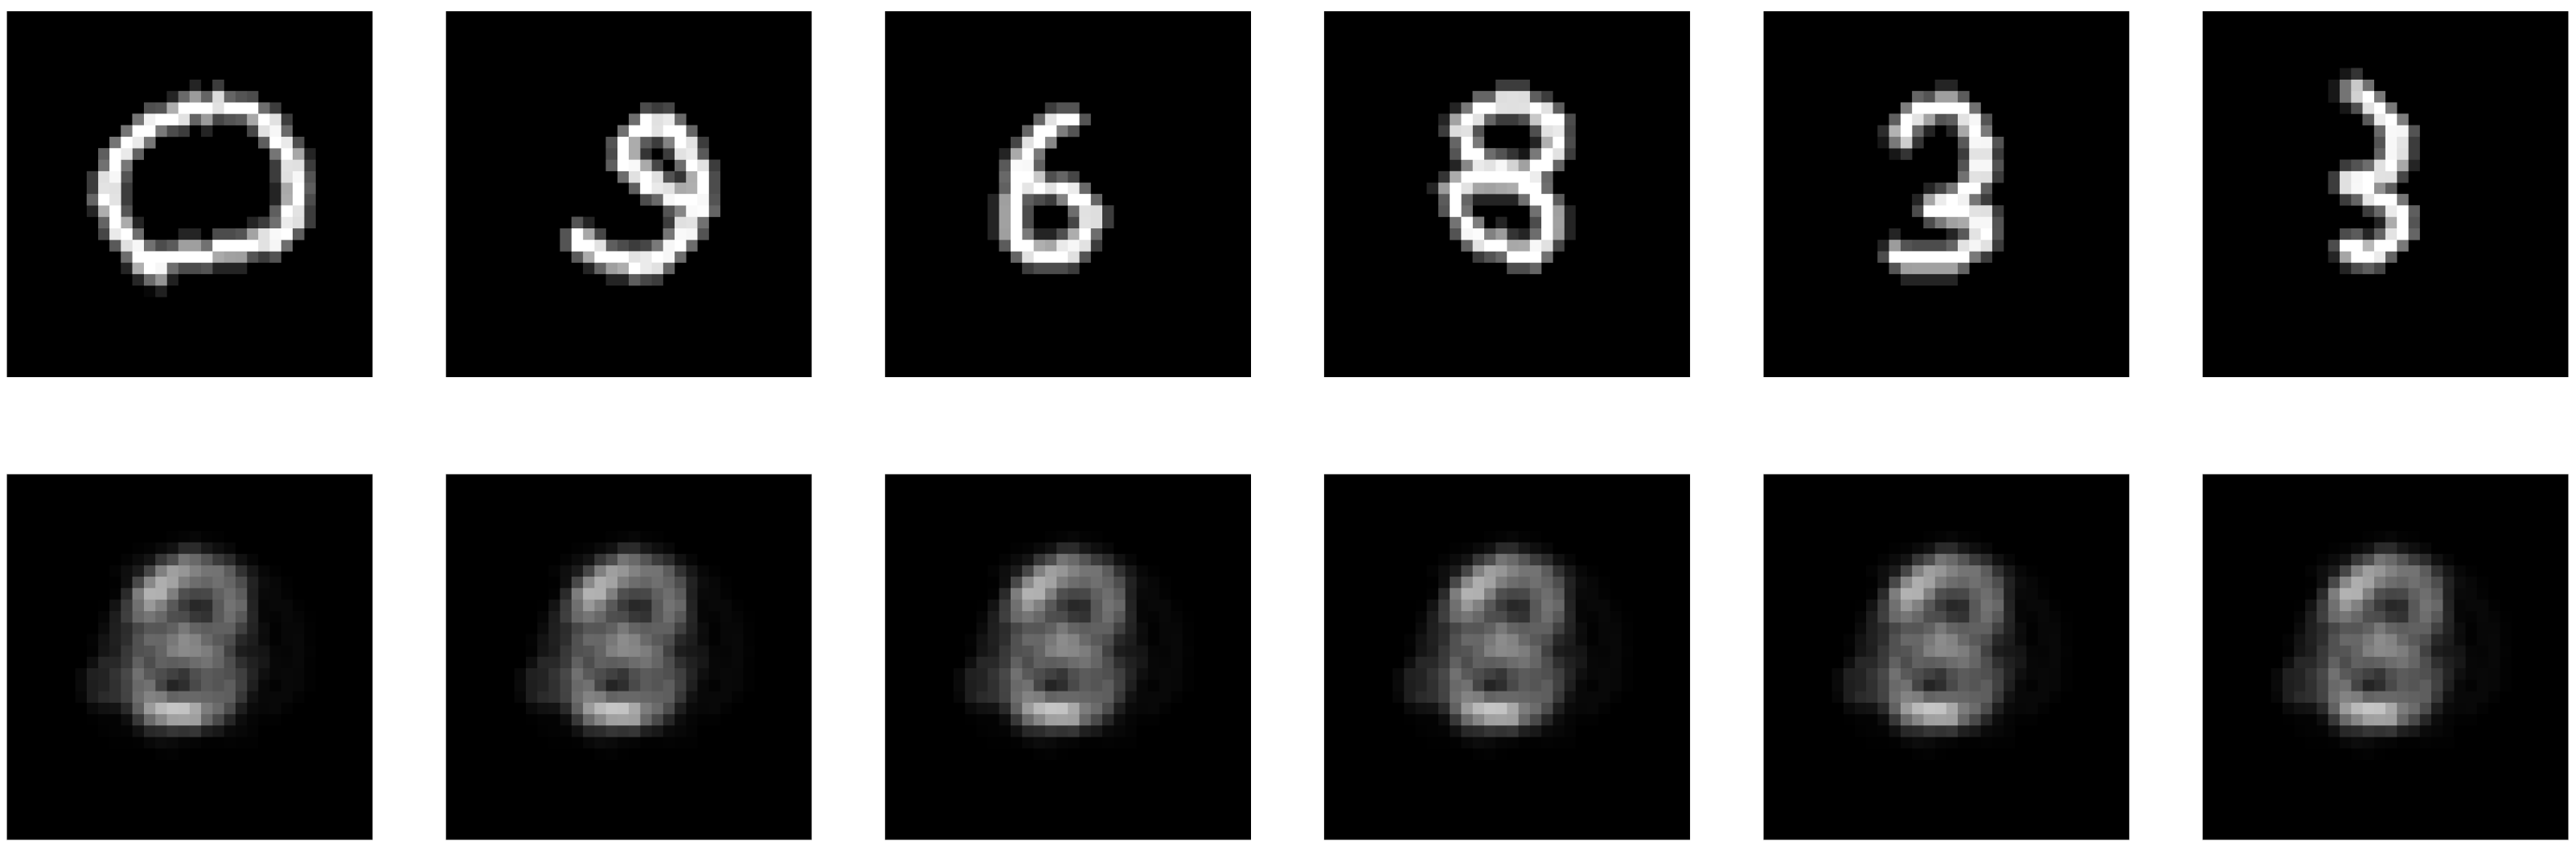
\includegraphics[width=0.7\linewidth]{Figures/FCHopfield1.png}
    \caption{The figure shows how, with a small value of $\beta$, each input gives the same output.}
\end{figure}

\begin{remark}
	$\left\|J_s\right\| = e_1$ where $e_1$ is the largest eigenvalue \\
	Also holds:  \begin{align*}
		\left\|J_s\right\| = e_1 = \text{Tr}\left(J_s\right) - \sum_{i=2}^{n} e_i = \sum_i p_i \text{Tr}\left((x^i-\bar{m})(x^i - \bar{m})^T\right) - \sum_{i=2}^{n} e_i = \sum_i p_i \left\|x^i -\bar{m}\right\|^2 - \sum_{i=2}^{n} e_i
	\end{align*}
	Thus, the bound presented in the previous proposition is high when other eigenvalues are small.
\end{remark}
The previous proposition states that we cannot properly use the Continuous Hopfield Neural Network if the temperature is too high, so it is necessary to formulate some condition for which the network has more than just one attractor point.
\begin{definition}[separation]
	Given a pattern matrix $X$, we define the pattern separation of the $i$-th pattern as:
	\[
	\Delta_i = \min_{j \neq i} (x^i)^Tx^i - (x^i)^T x^j
	\]
	Furthermore, an input $\xi$ is at least separated from $x^i$ while being separated from $x^j$ with $j \neq i$ if:
	\[
	i = \argmax_{k} \min_{j \neq k} (\xi^T x^k - \xi^Tx^j), \quad c =  \min_{j \neq i} (\xi^T x^i - \xi^Tx^j) > 0
	\]
\end{definition}
\begin{lemma}\text{from lemma.A4 in \cite{ramsauer2021hopfieldnetworksneed}}\\
	\label{lemma:Pattern_separation}
	If $\xi$ is at least separated from $x^i$ while being separated from all $x^j$ with $j \neq i$, then:
	\[
	\left\|x^i - f(\xi)\right\| \leq 2 \epsilon M
	\]
	where $M = \max_i \left\|x^i\right\|$ and $\epsilon = (P-1)e^{-\beta c}$
	\begin{proof}
		\begin{align*}
			\left[\softmax(\beta X^T \xi)\right]_i &= \frac{\exp(\beta x^i \xi)}{\sum_j \exp(\beta x^j \xi)} = \frac{1}{1 + \sum_{j\neq i} \exp(\beta \xi^Tx^j-\beta \xi^T x^i)} \geq \frac{1}{1 + \sum_{j\neq i} \exp(-\beta c)} \\
			&= \frac{1}{1 + (P-1) \exp(-\beta c)} = 1 - \frac{ (P-1) \exp(-\beta c)}{1 + (P-1) \exp(-\beta c)} \\
			&= 1 - \frac{\epsilon}{1 + (P-1) \exp(-\beta c)} \geq 1 - \epsilon
			\intertext{given k $\neq i$ then:}
			\left[\softmax(\beta X^T \xi)\right]_k &= \frac{\exp(\beta x^k \xi)}{\sum_j \exp(\beta x^j \xi)} = \frac{\exp(\beta \xi^Tx^k-\beta \xi^T x^i)}{1 + \sum_{j\neq i} \exp(\beta \xi^Tx^j-\beta \xi^T x^i)} \\
			&\leq \frac{\exp(-\beta c)}{1 + \sum_{j\neq i} \exp(\beta \xi^Tx^j-\beta \xi^T x^i)} \leq \exp(-\beta c) = \frac{\epsilon}{P-1}
		\end{align*}
		Now using the definition of $f$, we can prove the proposition:
		\begin{align*}
			\left\|x^i - f(\xi)\right\| &= \left\|x^i - X \softmax(\beta X \xi)\right\| = \left\|(1 - [\softmax(\beta X^T \xi)]_i) x^i - \sum_{k\neq i} x^k [\softmax(\beta X^T \xi)]_k\right\| \\
			&\leq \left(1 - \left[\softmax(\beta X^T \xi)\right]_i\right) \left\|x^i\right\| + \sum_{k\neq i} \left[\softmax(\beta X^T \xi)\right]_k \left\|x^k\right\| \\
			&\leq \epsilon M + \sum_{k\neq i} \frac{\epsilon}{P-1} M  = 2\epsilon M
		\end{align*}
	\end{proof}
\end{lemma}
The previous lemma suggests that separate patterns and $\beta$ not too small will make the sequence defined by the model closer to a particular pattern.
\begin{definition}
	\label{def:Si}
	Given a pattern matrix $X$ we define:
	\[
	S_i = \left\{ \xi \middle| \left\|\xi - x^i\right\| \leq \frac{1}{\beta P M}  \right\}
	\]
\end{definition}
\begin{proposition}\text{from lemma.A5 in \cite{ramsauer2021hopfieldnetworksneed}}\\
	\label{prop:local_conv}
	If $\xi \in S_i$ and $\Delta_i \geq \frac{2}{\beta P} + \frac{1}{\beta} \log(2(P-1)P \beta M^2)$ then: $f(\xi) \in S_i$
	\begin{proof}
		We define $\widetilde{\Delta_i}= \min_{j\neq i} \xi^Tx^i - \xi^T x^j$\\
		Using the  Cauchy-Schwartz inequality, we get: $\left|\xi^Tx^j - (x^i)^Tx^j\right| \leq \left\|\xi - x^i\right\|\, \left\|x^j\right\| \leq \left\|\xi - x^i\right\| M$

		\noindent So we can say that:
		\begin{align*}
			\widetilde{\Delta_i} &= \min_{j\neq i} \xi^Tx^i - \xi^T x^j =  \min_{j\neq i} \xi^Tx^i -\left(x^i\right)^Tx^i + \left(x^i\right)^Tx^i  -\xi^Tx^j + \left(x^i\right)^Tx^j - \left(x^i\right)^Tx^j \\
			&\geq \min_{j\neq i} \left(\left(x^i\right)^Tx^i - \left\|\xi - x^i\right\| M\right) - \left(\left(x^i\right)^Tx^j +\left\|\xi - x^i\right\| M\right) \\
			&= -2\left\|\xi -x^i\right\|M +  \min_{j\neq i} \left(x^i\right)^Tx^i - \left(x^i\right)^Tx^j = \Delta_i - 2\left\|\xi -x^i\right\|M  \\
			& \geq \Delta_i - \frac{2}{\beta P}
		\end{align*}
		Where the last inequality holds because  $\xi \in S_i$.\\
		From \cref{lemma:Pattern_separation} we can affirm that:
		\begin{align*}
			\|x^i - f(\xi)\| &\leq 2 \epsilon M = 2 M (P-1) \exp\left(-\beta \widetilde{\Delta_i}\right) \leq  2 M (P-1) \exp\left(-\beta \left(\Delta_i - \frac{2}{\beta P}\right)\right) \\
			&\leq 2 M \left(P-1\right) \exp\left(-\beta \left( \frac{2}{\beta P} + \frac{1}{\beta} \log\left(2\left(P-1\right)P \beta M^2\right) - \frac{2}{\beta P}\right)\right)\\
			&=  2 M \left(P-1\right) \frac{1}{2\left(P-1\right)P \beta M^2} = \frac{1}{\beta P  M}
		\end{align*}
	\end{proof}
\end{proposition}
Using the previous proposition and \cref{th:statonary_points} we can state that if the input is inside a sphere $S_i$, then the accumulation points, which are points of minima for the energy, are inside the sphere, which allows us to use the network properly, with the right choice of temperature, because different input gives different output.
\begin{remark}
	We can always find a value for $\beta$ that satisfies the condition of the previous proposition $\forall i$  solving:
	\[
	\min_i \Delta_i \geq \frac{2}{\beta P} + \frac{1}{\beta} \log(2(P-1)P \beta M^2)
	\]
	which is equivalent to solving:
	\[
	\beta \geq \frac{2}{P \min_i \Delta_i }+\frac{\log(2(P-1)P M^2)}{\min_i \Delta_i} +\frac{ \log(\beta)}{ \min_i \Delta_i}
	\]
	which solution is: $\beta \in (0,\beta_-] \cup [\beta_+,\infty)$ where $\beta_-,\beta_+$ are the point of \\intersection of $y=x$ and $y=\frac{2}{P \min_i \Delta_i }+\frac{\log(2(P-1)P M^2)}{\min_i \Delta_i} +\frac{ \log(x)}{ \min_i \Delta_i}$. \\
	For retrieval, the smallest solutions are useless because they correspond to the global convergence state of the network, as proved in \cref{prop:J_norm}. However, the largest ones are useful because they can give disjoint $S_i$.
\end{remark}

\begin{figure}[ht]
    \centering
    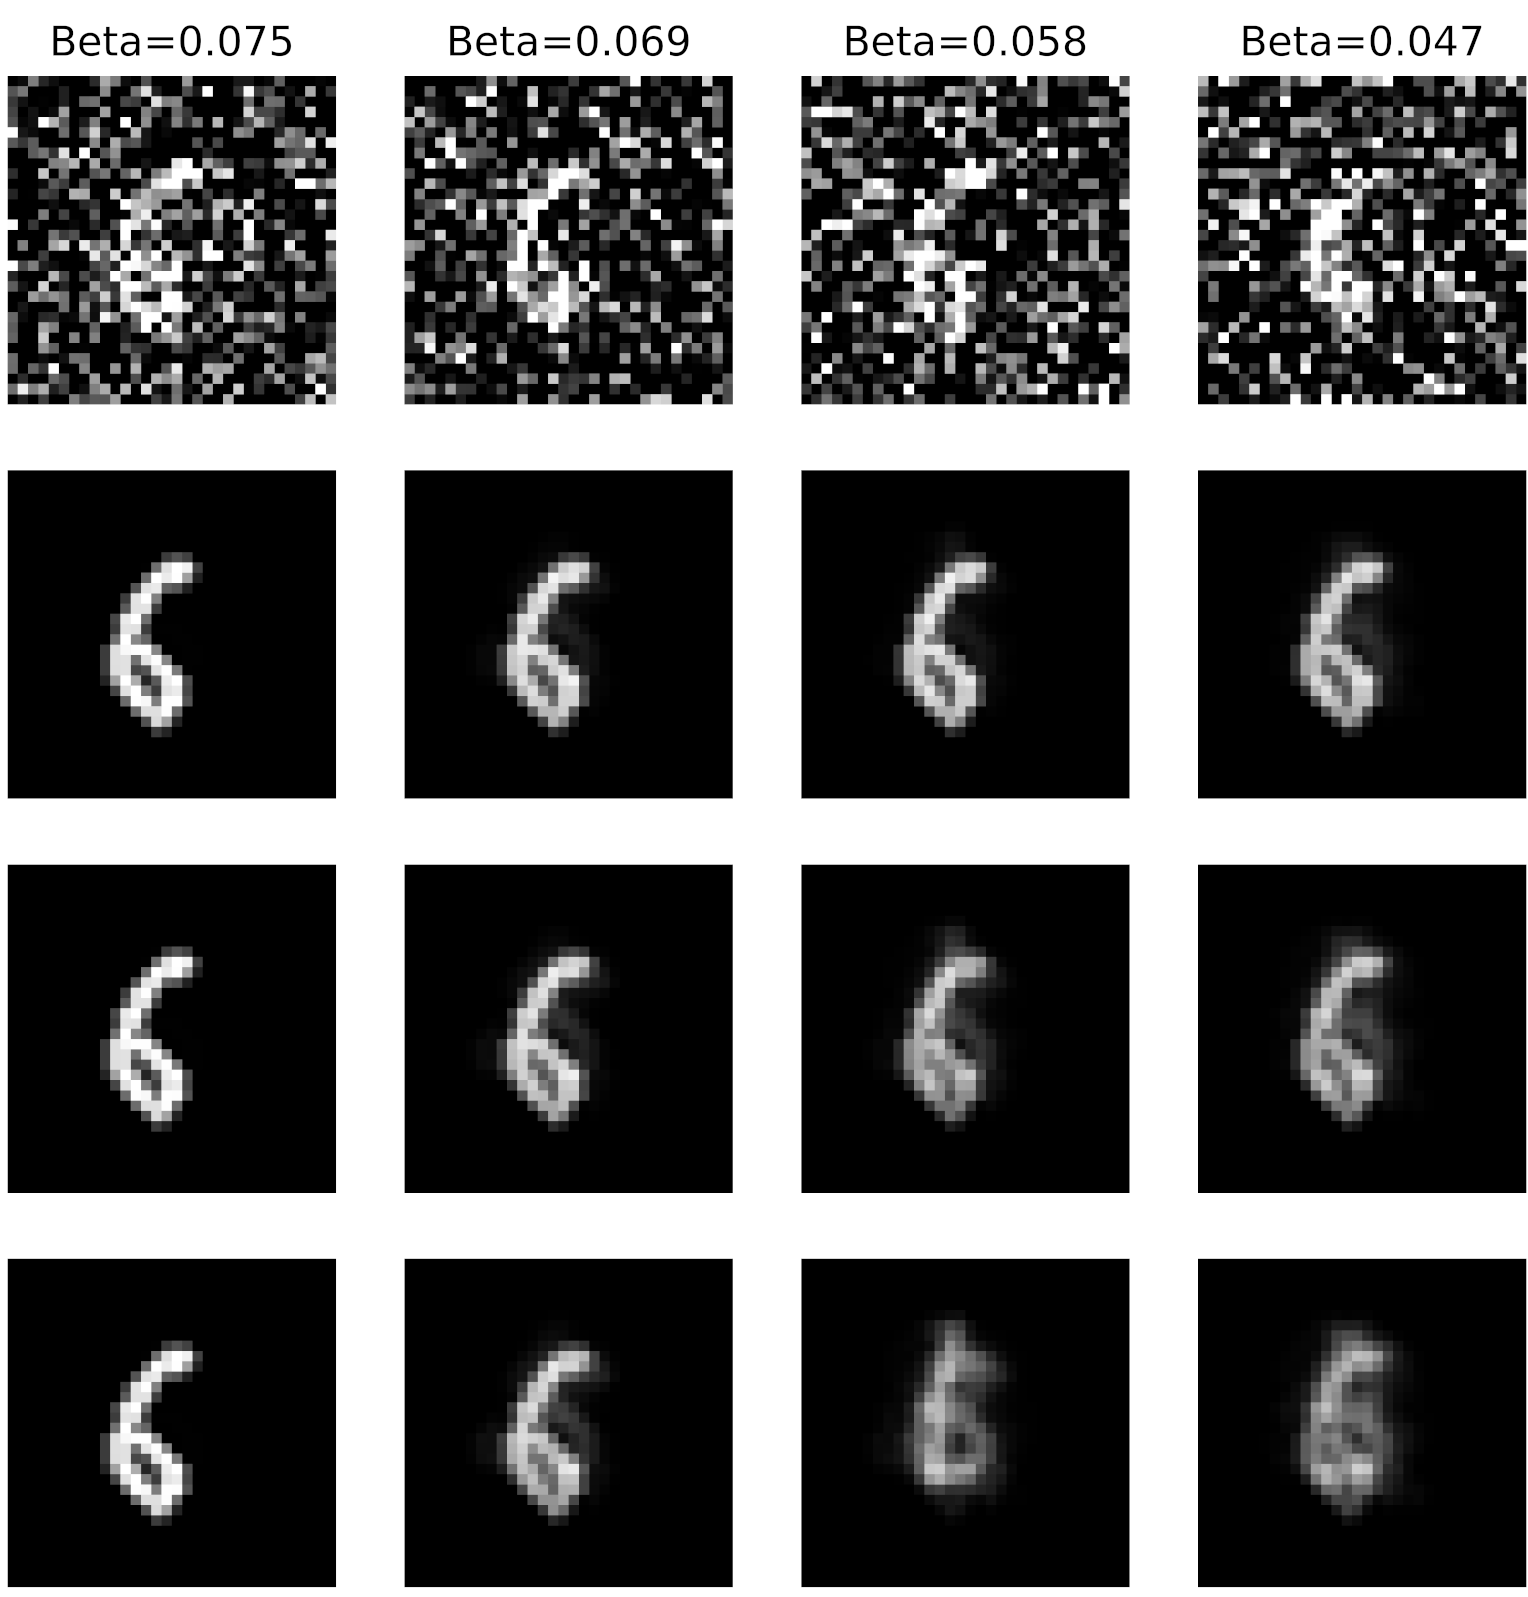
\includegraphics[width=0.6\linewidth]{Figures/FCHopfield.png}
    \caption{The figure shows how the same network gives different outputs with different $T$, larger values bring to a convergence point that is a mixed pattern instead smaller values give local convergence to the stored pattern. The input image is obtained as a random perturbation of a stored pattern.}
\end{figure}

\section{Comparison with discrete Hopfield network}
In this section we want to analyse the differences and analogies between the discrete and the continuum Hopfield networks.
\begin{itemize}
	\item \textbf{Network structure}\\
	Both networks receive an input image, represented as an array of numbers, and process it by correlation with stored patterns. By iteratively updating the input, each network aims to transform it into something closer to a stored pattern.
	\item \textbf{Energy minimization}\\
	An energy function can be defined for both networks, expressed in terms of correlations with stored patterns. This function decreases along the network dynamics and guides the system towards energy minima.
	\item \textbf{Stochasticity and temperature} \\
	Both networks have a parameter called temperature, which can be tuned to facilitate convergence. However, this parameter affects each network differently: in discrete networks, temperature controls the amount of random noise in the updating rule, introducing a degree of stochasticity. In continuous networks, the temperature affects how information is integrated within the softmax operation, so there is no randomness. Despite this difference, the two networks show similar behavior with respect to temperature. In both cases, high temperatures lead to uninformative outputs, where each input is transformed into a generic, uninformative result. Conversely, too low a temperature can also be problematic, leading to trivial outputs in both networks.
	\item \textbf{Pattern and training}\\
	In both networks, the energy function and update rules are defined in terms of stored patterns. However, due to the discrete nature of the neurons, the dynamics of discrete networks cannot be distinguished from the pattern vectors. In contrast, continuous networks allow the computation of derivatives, which allows them to be integrated into larger deep neural networks and trained with backpropagation. Discrete networks, on the other hand, lack any form of learning because the patterns are fixed and remain unchanged.
\end{itemize}
